%!TEX root = main.tex

\section{Model Improvements}
\label{sec:improvements}

Having a solid baseline model for our malware detection task together with how laboratory \textit{vs.}\ real-world scenarios change the model outcome, we now take this section to present the improvements made in order to obtain a more robust model to detect malware.
We start by describing our first improvement, applying a multi layer model to extract more information regarding a sample.
We then take this enhanced model and increase the number of features to include dynamic content and how it impacted the model's results.

%%%%%%%%%%%%%%%%%%%%%%%%%%%%%%%%%%%%%%%%%%%%%%%%%%%%%%%%%%%%%%%%%%%%%%%%
\subsection{Multi Layer Model}
\label{section:improvements_multi_layer}

On the previous chapter we ended up with a simple \gls{lr} model $\LR$ that given a set of static imports from a sample, would give the probability of it being malware.

In this section we provide a new model $\mathcal{E}$ comprises a simple ensemble stacking approach, which instead of using a single \gls{lr} classifier, multiple ones are used, layered into two steps.

The first step (layer $\mathcal{E}_{\mathcal{L}_{0}}$) is composed of $n$ \gls{lr} models, where $n$ is the number of possible classes.
Each model is trained to output the likelihood of sample belonging to one of the $n$ classes, in a \textit{one-vs-all} methodology (\ie\ a sample either belongs to $\mathcal{C}_{n}$ or not), having as input the raw features (\eg\ static imports).

The second step (layer $\mathcal{E}_{\mathcal{L}_{1}}$) is identical to $\mathcal{LR}$, but now takes as features the output of each classifier from the previous layer, outputting the likelihood of a sample being malware.

In summary, as depicted in Figure \ref{fig:dia_multilayer}, we define a 2 layer ensemble stacking with $n$ classifiers on the first layer to a single classifier in the second layer.

\begin{figure}[h]
	\centering
	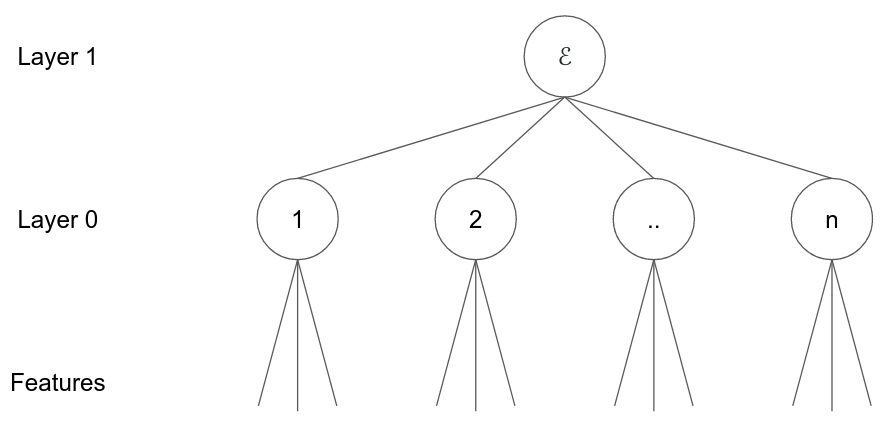
\includegraphics[width=\columnwidth]{dia_multilayer}
	\caption{Multi layer model representation.}
	\label{fig:dia_multilayer}
\end{figure}

%%%%%%%%%%%%%%%%%%%%%%%%%%%%%%%%%%%%%%%%%%%%%%%%%%%%%%%%%%%%%%%%%%%%%%%%
\subsection{Malware Classes}

We now present our approach on selecting the $n$ classes of interest.
This represents another labeling problem, but now instead of having to label between goodware and malware, we have to label the malware as belonging to some subclass.

With this in mind, we chose 6 malware classes: \textit{virus}, \textit{trojan}, \textit{worm}, \textit{ransom}, \textit{spyware} and \textit{other}.

To help label our malware samples into the aforementioned classes, we take a tool by Sebastián, M. et al.~\cite{sebastian2016avclass}, AVClass, which was built to normalize a malware sample name into the most likely family, and modify it such that instead of providing a family name, it would provide one (or more) of the 6 previously defined classes.
Specifically, we changed it in a way that given a set of malware names, the output would be a distribution over the 6 malware classes.

To calculate each class weight we apply the following formula
\begin{eqnarray*}
	\mathcal{W}_c = \dfrac{f_c}{\sum\limits_{c}f_c}
\end{eqnarray*}

where $f_c$ is the frequency for the class $c$ and $\sum_{c}f_c$ is the number of times all classes appear.
For example, if a given set of names contain the name \textit{trojan} 3 times and the name \textit{virus} one time, then the weights would be

\begin{eqnarray*}
	\mathcal{W}_{trojan}=\dfrac{3}{4}=0.75,~\mathcal{W}_{virus}=\dfrac{1}{4}=0.25,\\\mathcal{W}_{c}=0, c \in \{worm, spyware, other, ransom\}
\end{eqnarray*}

\medskip

Having these malware classes defined for our multi layer model, we also added the \textit{goodware} class for samples that are not malware.
Doing so gives us 7 possible classes, 6 of which are malware only.
It is worth mentioning that if a sample belongs to the \textit{goodware} class, it cannot belong to any other, likewise, if it belongs to any malware class, it cannot belong to the \textit{goodware} class.
Table \ref{tab:dataset_sizes_new} discriminates the amount of each malware class.

\begin{table}[!htb]
	\renewcommand{\arraystretch}{1.2} % more space between rows
	\centering
	\begin{tabular}{lccc}
		Dataset			& $\CC_{real}$ & $\CC_{loose}$ & $\CC_{strict}$	\\
		\hline
		Trojan			& 97,054 & 44,329 & 24,176\\
		Other			& 49,443 & 24,126 & 14,750\\
		Worm			& 24,554 & 14,837 & 9,381\\
		Virus			& 21,055 & 12,531 & 6,899\\
		Spyware			& 20,724 & 10,172 & 5,955\\
		Ransom			& 7,761 & 1,924 & 1,160\\
		\hline
		\hline
		Malware Total	& 98,582 & 45,306 & 24,658\\
		\hline
	\end{tabular}
	\medskip
	\caption{Samples belonging to each of the 6 malware classes for $\CC_{real}$, $\CC_{loose}$ and $\CC_{strict}$.}
	\label{tab:dataset_sizes_new}
\end{table}

\medskip

In the base model, we used static imports as features for our malware detection model.
Although the results are reasonable, the information which can be retrieved from static imports alone is limited.
As an example, if a sample is compressed, encrypted or packed, its behavior cannot be inferred from static imports only.
To overcome these limitations, we resort to more dynamic information provided by Cuckoo.

%%%%%%%%%%%%%%%%%%%%%%%%%%%%%%%%%%%%%%%%%%%%%%%%%%%%%%%%%%%%%%%%%%%%%%%%
\subsection{Category Calls}
\label{section:improvements_categories}

The first type of dynamic information we extracted were the number of dynamic category calls.
When Cuckoo runs and monitors a sample, it registers some low level library calls, which it then assigns to a fixed number of categories.

There are a total of 14 different categories defined by Cuckoo: \textit{anomaly}, \textit{device}, \textit{filesystem}, \textit{hooking}, \textit{misc}, \textit{network}, \textit{process}, \textit{registry}, \textit{services}, \textit{socket}, \textit{synchronization}, \textit{system}, \textit{threading} and \textit{windows}.
After using Celery~\cite{tool:celery} to extract the number of each category calls for the samples, we obtained a total of 148,036 samples with information regarding category calls.

To normalize the category calls value, we decide to transform the values to follow a normal distribution.
We do this by using scikit-learn's~\cite{tool:sklearn} \textit{QuantileTransformer} with a normal distribution, which splits the possible values into bins such that the resulting distribution is of type \textit{Gaussian} with a mean of 0.
This way we have a greater number of bins around the mean, allowing for better discrimination, whereas very large values fall into the same bin.

%%%%%%%%%%%%%%%%%%%%%%%%%%%%%%%%%%%%%%%%%%%%%%%%%%%%%%%%%%%%%%%%%%%%%%%%
\subsection{Library Calls}
\label{section:improvements_api_unigrams}

Our second type of dynamic information are the number of library calls.
While \textit{category calls} provide the number of calls for a given category, \textit{library calls} provide the count for each library call, hence being a subset of the previous.

Cuckoo~\cite{tool:cuckoo} registers the number of calls for 163 different functions, ranging from opening and closing files, to opening and closing sockets.
Again we used Celery~\cite{tool:celery} to extract these numbers, obtaining information from 148,036 samples.

Given we are dealing with a high number of features (163 different library calls), we decided to apply the same variance threshold as in Section \ref{section:feature_selection}, to remove features that do not vary in most samples.
By choosing a threshold of 80\%, we remove library calls that do not vary in more than 80\% of the samples, effectively reducing the number of library calls to 144.
With regards to how these features can vary from 0 to $+\infty$, as before, we again apply a quantile transformer with a normal distribution.

%%%%%%%%%%%%%%%%%%%%%%%%%%%%%%%%%%%%%%%%%%%%%%%%%%%%%%%%%%%%%%%%%%%%%%%%
\subsection{Cuckoo Signatures}
\label{section:improvements_signatures}

For our third and last type of dynamic information, we resort to Cuckoo's~\cite{tool:cuckoo} custom signatures.
These signatures are built from certain activities that Cuckoo deems malicious or suspicious.
For example, if a sample allocates memory and then makes it executable, it might suggest some sort of packing or obfuscation.

To extract these signatures, we use Celery~\cite{tool:celery} and obtain a total of 124,821 samples and 61 different signatures.
As with our static import features, we use a binary vector for each sample, where each position corresponds to a specific signature. Re-iterating on how we represent this, if a given signature $i$ is present in a sample, its feature vector $x$ will have the value 1 at that position $x_i$. Likewise, if a given signature $j$ is not present in a sample, its feature vector $x$ will have the value 0 at that position $x_j$.

\medskip

We joined these features $\FF_{dynamic}$ to the labeled samples $\CC_{real}$, obtaining a total of 122,633 labeled samples with the new features $\DD_{dynamic} = \CC_{real} \cap \FF_{dynamic}$.

Given there is a lower amount of available samples, we provide in Table \ref{tab:dataset_sizes_improved} the new sizes for $\CC_{real}$, $\CC_{loose}$ and $\CC_{strict}$, which take into account the new features $\FF_{dynamic}$.

\begin{table}[!htb]
	\renewcommand{\arraystretch}{1.2} % more space between rows
	\centering
	\begin{tabular}{lccc}
		Dataset			& $\CC_{real}$ & $\CC_{loose}$ & $\CC_{strict}$	\\
		\hline
		Malware			& 94,248 & 42,911 & 23,437\\
		Goodware		& 28,385 & 1,741 & 1,741\\
		\hline
		Total			& 122,633 & 44,652 & 25,178\\
		\hline
	\end{tabular}
	\medskip
	\caption{New sizes for datasets $\CC_{real}$, $\CC_{loose}$ and $\CC_{strict}$.}
	\label{tab:dataset_sizes_improved}
\end{table}

%%%%%%%%%%%%%%%%%%%%%%%%%%%%%%%%%%%%%%%%%%%%%%%%%%%%%%%%%%%%%%%%%%%%%%%%
\section{Improved Model Results}
\label{section:improvements_results}

We now present the results of our new model $\mathcal{E}$, validated using the same methodology as described in \ref{sec:eval_results}.

Specifically we test the model using the baseline cross-validation methodology, followed by our three temporally consistent scenarios: \textit{Past-to-Present}, \textit{Present-to-Past} and \textit{Temporal Window}.
We test each methodology using the three different scenarios: $\mathcal{S}_{\strict}$, $\mathcal{S}_{\loose}$ and $\mathcal{S}_{\real}$.
\medskip

Starting with \textit{laboratory conditions}, we apply the cross-validation evaluation to model $\mathcal{E}$ with the labeled dataset $\CC_{strict}$ and features $\DD_{dynamic}$, providing scenario $\mathcal{S}_{\strict}$.
For this scenario, we obtain an \gls{auroc} of 98\%, as presented by the red curve in Figure \ref{fig:improved_xval}.

Relaxing to more \textit{real-world conditions}, under the form of a less reliable ground truth, we test the datasets $\CC_{loose}$ and $\CC_{real}$ on features $\DD_{dynamic}$.
As shown in Figure \ref{fig:improved_xval}, the score under \gls{auroc} is 98\% for $\mathcal{S}_{\loose}$ (blue curve) and 95\% for $\mathcal{S}_{\real}$ (green curve).

\begin{figure}[!h]
	\centering
	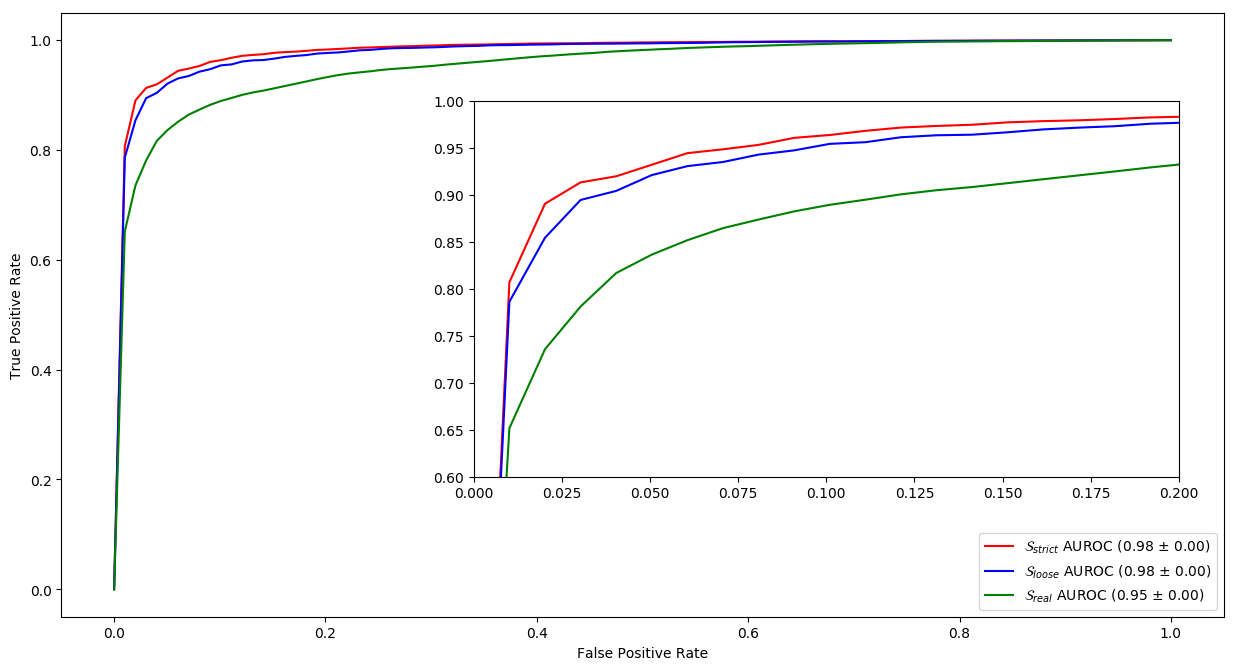
\includegraphics[width=\columnwidth]{xval_improved}
	\caption{Multi layer results for dynamic features in laboratory conditions.}
	\label{fig:improved_xval}
\end{figure}

% Adicionar seccao para resultados do multi layer apenas.

As with previous results, one notes that from $\mathcal{S}_{\strict}$ to $\mathcal{S}_{\loose}$ the results are not affected at all, when the change between the scenarios is merely in the number of malware samples.
Between $\mathcal{S}_{\loose}$ to $\mathcal{S}_{\real}$ we again note the already seen pattern, the score is lowest when using the most realistic dataset.

The comparison between scenarios does not yield any new information from what was seen in Section \ref{section:single_layer_results}.
What is more interesting is that the absolute values are boosted in all scenarios, which show indeed that using the multi-layer approach with dynamic features improve the model's results.

Having applied the same cross-validation to our modified model, obtaining interesting results, we now go over to test how our temporal based methodologies are affected.

\medskip

We start again with \textit{Past-to-Present} validation to each scenario $\mathcal{S}_{\strict}$, $\mathcal{S}_{\loose}$ and $\mathcal{S}_{\real}$.
Figure \ref{fig:pastpresent_modified} shows the \gls{auroc} at every iteration (\ie\ fold) for each scenario: 96\% for $\mathcal{S}_{\strict}$ and $\mathcal{S}_{\loose}$, and 92\% $\mathcal{S}_{\real}$.

\begin{figure}[!htb]
	\centering
	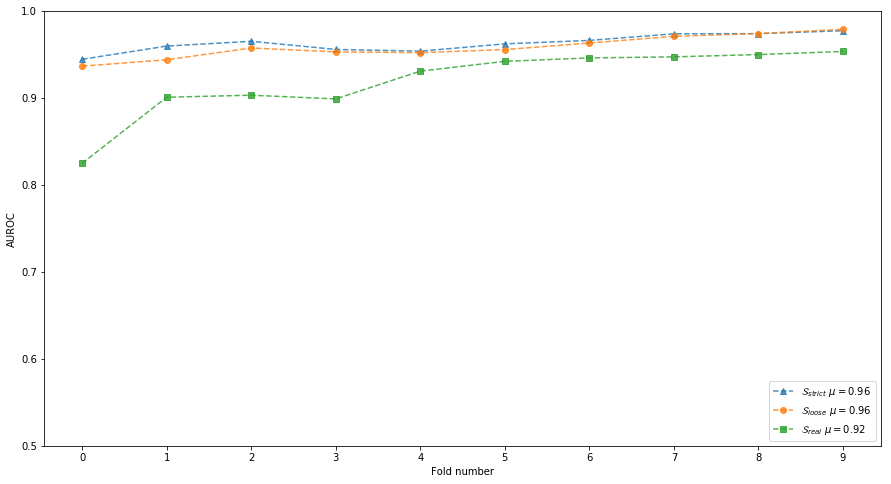
\includegraphics[width=\columnwidth]{pastpresent_improved}
	\caption[Multi layer results for dynamic features in \textit{Past-to-Present}.]{\gls{auroc} for each iteration of the \textit{Past-to-Present} evaluation. Folds order consistent with temporal order (\ie\ fold 0 contains older samples than
		fold 1)}
	\label{fig:pastpresent_modified}
\end{figure}

When comparing the average \gls{auroc} between cross-validation and \textit{Past-to-Present} validation, we note that both $\mathcal{S}_{\strict}$ and $\mathcal{S}_{\loose}$ decrease 2\%, while $\mathcal{S}_{\real}$ decreases 3\%.
This decrease is not a surprise, given the temporal consistency enforcement between samples.

The results are consistent with was previously seen in Section \ref{section:single_layer_results}, with the added factor that the absolute values are higher, and the tendency to increase is more present as we move forward in time, close to the validation set.

\medskip

Following the previous evaluation order, we now present the results using our \textit{Present-to-Past} validation methodology.
In Figure \ref{fig:presentpast_improved} we present the \gls{auroc} for each iteration, where higher folds represent older samples. Here we see values of 97\% for $\mathcal{S}_{\strict}$, 98\% for $\mathcal{S}_{\loose}$ and 96\% $\mathcal{S}_{\real}$.

\begin{figure}[!h]
	\centering
	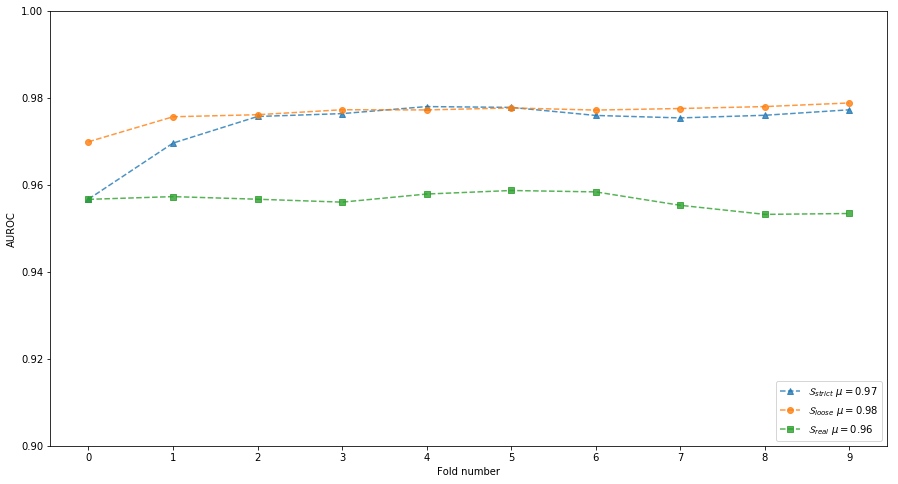
\includegraphics[width=\columnwidth]{presentpast_improved}
	\caption[Multi layer results for dynamic features in \textit{Present-to-Past}.]{\gls{auroc} for each iteration of the \textit{Present-to-Past} evaluation. Folds order is the inverse of temporal order (\ie\ fold 0 contains newer samples than fold 1)}
	\label{fig:presentpast_improved}
\end{figure}

When comparing to cross-validation, we note $\mathcal{S}_{\strict}$ is affected as expected, whereas $\mathcal{S}_{\loose}$ is not.
The fact that the datasets vary in size and so the amount of goodware and malware used for testing in each may vary, can justify how the $\mathcal{S}_{\loose}$ is not affected, whereas $\mathcal{S}_{\strict}$ is.

$\mathcal{S}_{\real}$ seems to have a higher value than in cross-validation, but it is rounded, which slightly inflates the value.
In practice both cross-validation and \textit{Present-to-Past} are identical for $\mathcal{S}_{\real}$.

In these results, the noticeable increase in the first 3 folds (0, 1 and 2) for $\mathcal{S}_{\strict}$ and $\mathcal{S}_{\loose}$ goes even more in favor with our argument that samples closer to the validation set benefit the model.
More so as the \gls{auroc} stabilizes from those folds on.
This effect is not as accentuated for $\mathcal{S}_{\real}$, although using more and older folds do not provide significantly better results.

\medskip

Finally, we retest how a reduced training set behaves in our scenarios by using our \textit{Temporal Window} methodology.
As previously mentioned, the first 3 folds seem to provide enough information to obtain good results, hence we apply the same sliding window size of $n=3$ as in Section \ref{section:single_layer_results}.
Starting at the oldest fold, we apply this window and slide it by one fold at each iteration.
Figure \ref{fig:slidingwindow_modified} shows how all our scenarios $\mathcal{S}_{\strict}$, $\mathcal{S}_{\loose}$ and $\mathcal{S}_{\real}$ score the same \gls{auroc} of 94\%, although with different curves.

For $\mathcal{S}_{\strict}$, $\mathcal{S}_{\loose}$ the score is equally and negatively affected by 4\%.
The jagged curve on both scenarios indicate that slight changes on the \gls{fpr} threshold have significant impact on the \gls{tpr}, this may be caused by the smaller dataset size, which in turn creates uneven folds for malware and goodware.

\begin{figure}[!h]
	\centering
	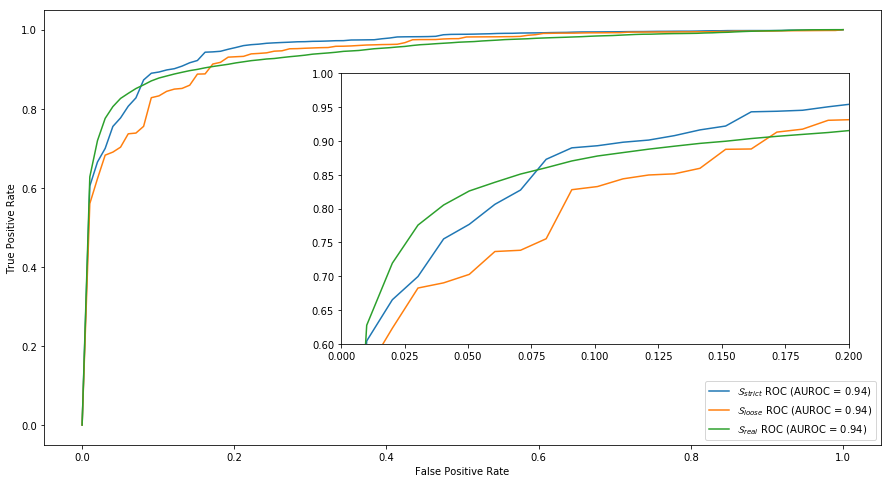
\includegraphics[width=\columnwidth]{Figures/slidingwindow_improved.png}
	\caption[Multi layer results for dynamic features in \textit{Temporal Window}.]{\gls{auroc} for our three scenarios, under the \textit{Temporal Window} methodology.}
	\label{fig:slidingwindow_modified}
\end{figure}

For $\mathcal{S}_{\real}$, the fact that it only loses 1\% when compared to cross-validation shows that indeed our argument about reducing the training set size is sustained.
Its curve is much smoother when compared to the previous scenarios, as the dataset is bigger and more even.

\medskip

%As a closing remark, we reaffirm on how it is possible to yield reasonable results when considering temporal consistent samples, specifically in this improved model, which not only uses more features, but has the ability to provide more information regarding a malware sample, as it can discriminate malware classes due to its multi layer design.
The improved layer results are summarized in Table \ref{tab:multilayer_results}.

\begin{table}[!htb]
	\renewcommand{\arraystretch}{1.2} % more space between rows
	\centering
	\begin{tabular}{ccccc}
		AUROC & $\DS_\strict$ & $\DS_\loose$ & $\DS_\real$ & Train/Test \%\\
		\hline
		Cross-Validation & 0.98 & 0.98 & 0.95 & 90 / 10\\
		Past-to-Present & 0.96 & 0.96 & 0.92 & 10 to 90 / 10\\
		Present-to-Past & 0.97 & 0.98 & 0.96 & 10 to 90 / 10\\
		Sliding-Window & 0.94 & 0.94 & 0.94 & 30 / 10\\
		\hline
	\end{tabular}
	\medskip
	\caption{Multi layer results summary.}
	\label{tab:multilayer_results}
\end{table}
